
\documentclass[template=tabling,81pt,headonall]{azmoon}
\usepackage{xepersian}
\usepackage{amsfonts}
\usepackage{graphicx}
\graphicspath{ {./images/} }
\settextfont{Yas}
\setdigitfont{A Iranian Sans}
\usepackage{fontawesome5}

\printanswers
    \teacher{محمد صالح علی اکبری}
    \teachertitle{دبیر}
    \city{گناباد}
    \schooltitle{متوسطه دوره دوم}
    \school{شاهد امام (ره)}
    \grade{دهم}
    \branch{۱۵۱}
    \topic{ریاضی}
    \examdate{07/09/1402}
    \answertime{40 دقیقه}
    \begin{document}
	\begin{questions}
		\nointerlineskip%
		\vskip-\baselineskip
		\question[0.5]{%
خط $l$ و نقطه $A$ خارج از خط $l$ مفروض است. چند خط از این نقطه می‌گذرد که بر خط $l$ عمود است؟}\question[1]{%
عکس هر یک از گزاره‌های زیر را بنویسید.
    \begin{parts}[1]\part{عدد $2$ فرد است.}
\part{مجموع زوایای یک مثلث $180$ درجه است.}
\end{parts}

    }\question[1.5]{%
روش رسم خطی موازی به فاصله ۳ واحد از خطی دیگر به کمک پرگار و خط کش را توضیح دهید.}\question[2]{%
فرض کنید که برای لوزی بودن یک چهارضلعی کافی است که قطرهای آن چهارضلعی عمود منصف یک دیگر باشند. لوزی رسم کنید که طول ضلع آن 10 و ارتفاع بزرگ آن دو برابر ارتفاع کوچک آن باشد.(روش رسم با خط کش و پرگار توضیح داده شود.)}\question[2]{%
اثبات کنید عمود منصف‌های مثلث همرس اند.}\question[2]{%
اثبات کنید نیمسازهای مثلث همرس اند.}\question[2]{%
روش پیدا کردن مرکز یک دایره که فقط یک کمان از آن در دسترس است را توضیح دهید. (خط کش و پرگار تنها ابزار در دسترس است)}\question[5]{%
قضیه: اگر در مثلثی دو ضلع نابرابر باشند، زاویه روبه‌رو به ضلع بزرگتر است از زاویه روبه‌رو به ضلع کوچک‌تر. \\ 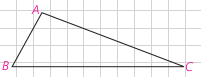
\includegraphics[scale = 0.48]{Screenshot from 2023-11-25 20-08-09} \\ فرض: $AB<AC$ \\ حکم: $\hat{C} < \hat{B}$\\الف) قضیه فوق را اثبات کنید.\\ب)عکس قضیه فوق را بنویسید.\\ج)عکس قضیه فوق را اثبات کنید.}\question[2]{%
صحت گزاره‌های زیر را بررسی کنید در صورت اشتباه بودن مثال نقض ارائه کنید.
    \begin{parts}[1]\part{در تمام مثلث‌ها نقطه تقاطع عمود منصف‌ها داخل مثلث است.}
\part{در هیچ مثلثی عمودهای مثلث بر اضلاع آن منطبق نمی‌شود.}
\part{میانه ساق‌های مثلث متساوی الساقین‌همیشه هم دیگر را بیرون مثلث قطع می‌کنند.}
\part{عمود منصف‌های هر دو وتر از یک دایره فقط در مرکز دایره هم دیگر را قطع می‌کنند.}
\end{parts}

    }\question[2]{%
قضیه زیر را به کمک برهان خلف اثبات کنید:\\قضیه: از هر نقطه غیر واقع بر یک خط نمی‌توان بیش از $2$ خط بر آن خط عمود رسم کرد.}\end{questions}
    \end{document}
    